\documentclass[11pt,a4paper]{article}

% Packages
\usepackage[utf8]{inputenc}
\usepackage[margin=0.9in]{geometry}
\usepackage{amsmath,amssymb}
\usepackage{graphicx}
\usepackage{booktabs}
\usepackage{hyperref}
\usepackage{xcolor}
\usepackage{enumitem}
\usepackage{tcolorbox}
\usepackage{multicol}

% Colors
\definecolor{firecolor}{RGB}{231, 76, 60}
\definecolor{warningcolor}{RGB}{243, 156, 18}
\definecolor{infocolor}{RGB}{52, 152, 219}

% Hyperlinks
\hypersetup{
    colorlinks=true,
    linkcolor=firecolor,
    urlcolor=infocolor,
    citecolor=firecolor
}

% Title
\title{
    \textbf{\LARGE 111 Years of California Wildfires} \\
    \vspace{0.3cm}
    \large What 23 Million Acres and 5,575 Fires Reveal About \\
    Patterns, Methods, and the Path Forward
}
\author{
    \textbf{FireAnalyst Research Project} \\
    \small Statistical Analysis of California Fire Perimeters (1912--2023) \\
    \vspace{0.2cm}
    \small \href{https://github.com/ngrief/FireAnalyst}{github.com/ngrief/FireAnalyst}
}
\date{\today}

\begin{document}

\maketitle

\begin{tcolorbox}[colback=infocolor!5!white, colframe=infocolor, title=\textbf{Executive Summary}]
This analysis examines 111 years of California wildfire data using rigorous statistical methods. Key findings include significant temporal and seasonal patterns, identification of primary ignition sources, and critical evaluation of containment effectiveness metrics. Importantly, this work identifies fundamental methodological limitations in standard effectiveness measures and proposes evidence-based improvements. All code, data, and methodology are open-source and reproducible.
\end{tcolorbox}

\vspace{0.3cm}

%=====================================
\section{The Scale of the Problem}
%=====================================

California's wildfire challenge is immense. This analysis spans \textbf{1912 to 2023}, examining \textbf{5,575 validated fire incidents} that burned \textbf{23.4 million acres}---an area larger than Indiana.

\subsection{Key Statistics}

\begin{multicols}{2}
\textbf{Fire Sizes:}
\begin{itemize}[leftmargin=*]
    \item \textbf{Mean:} 4,195 acres
    \item \textbf{Median:} 127 acres
    \item \textbf{Maximum:} 1,032,700 acres
    \item \textbf{95th percentile:} 13,841 acres
    \item \textbf{99th percentile:} 83,193 acres
\end{itemize}

\textbf{Containment Duration:}
\begin{itemize}[leftmargin=*]
    \item \textbf{Average:} 16 days (383 hours)
    \item Distribution highly right-skewed
    \item Some fires: $<$24 hours
    \item Megafires: weeks to months
\end{itemize}
\end{multicols}

The extreme difference between mean (4,195 acres) and median (127 acres) reveals a critical pattern: \textbf{most fires are small, but a few are catastrophic}. This right-skewed distribution drives policy challenges---you can't prepare for the average fire; you must prepare for the worst.

%=====================================
\section{What the Data Reveals}
%=====================================

\subsection{Temporal Trends: Fire Activity is Increasing}

Statistical testing confirms what fire managers have observed: \textbf{fire activity shows a significant increasing trend} (linear regression, $p < 0.001$).

\textbf{Peak years for fire occurrence:}
\begin{itemize}
    \item \textbf{2017:} 319 fires (record high)
    \item \textbf{2008:} 292 fires
    \item \textbf{2020:} 249 fires
    \item \textbf{2018:} 220 fires
    \item \textbf{2021:} 214 fires
\end{itemize}

\textbf{Notice:} All top-5 years occurred in the 21st century, with \textbf{four of the five since 2017}. The 2010s decade recorded 1,819 fires---the highest of any decade in the dataset.

\begin{figure}[h]
\centering
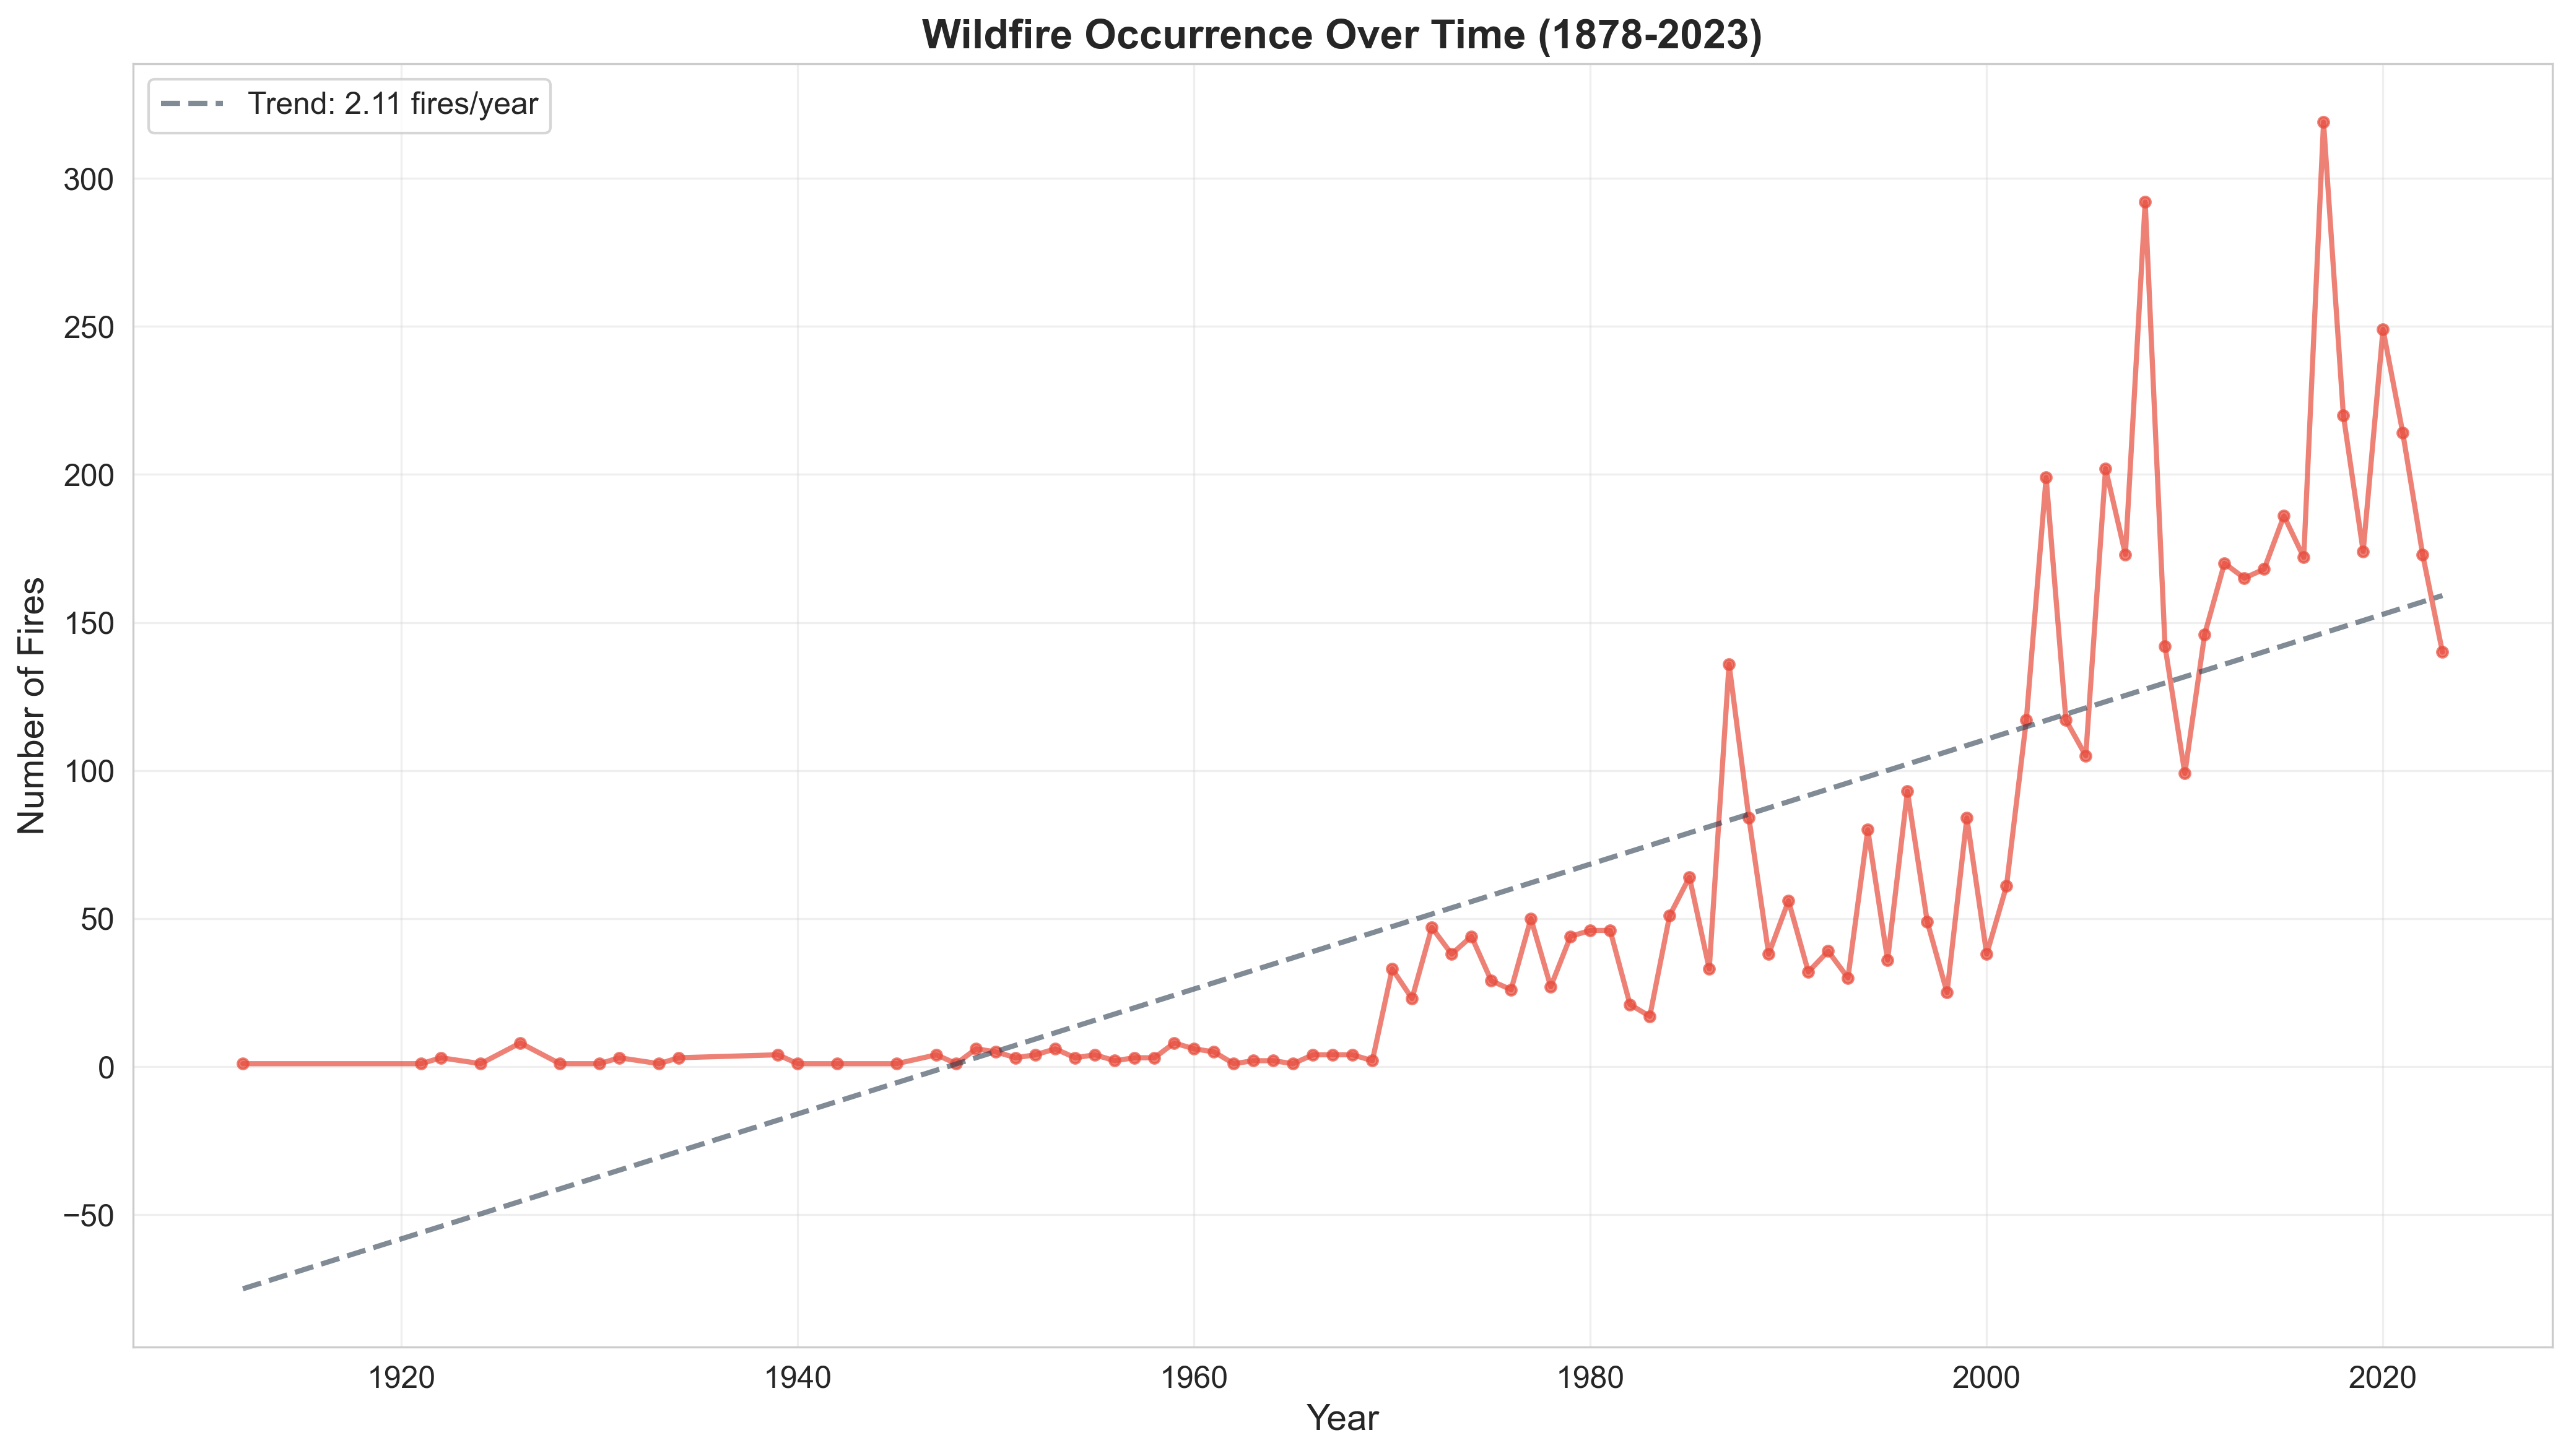
\includegraphics[width=0.85\textwidth]{fires_over_time.png}
\caption{Wildfire occurrence from 1912--2023 showing significant increasing trend. The trend line confirms statistically significant growth in fire activity, particularly accelerating in the 21st century.}
\label{fig:temporal}
\end{figure}

\begin{figure}[h]
\centering
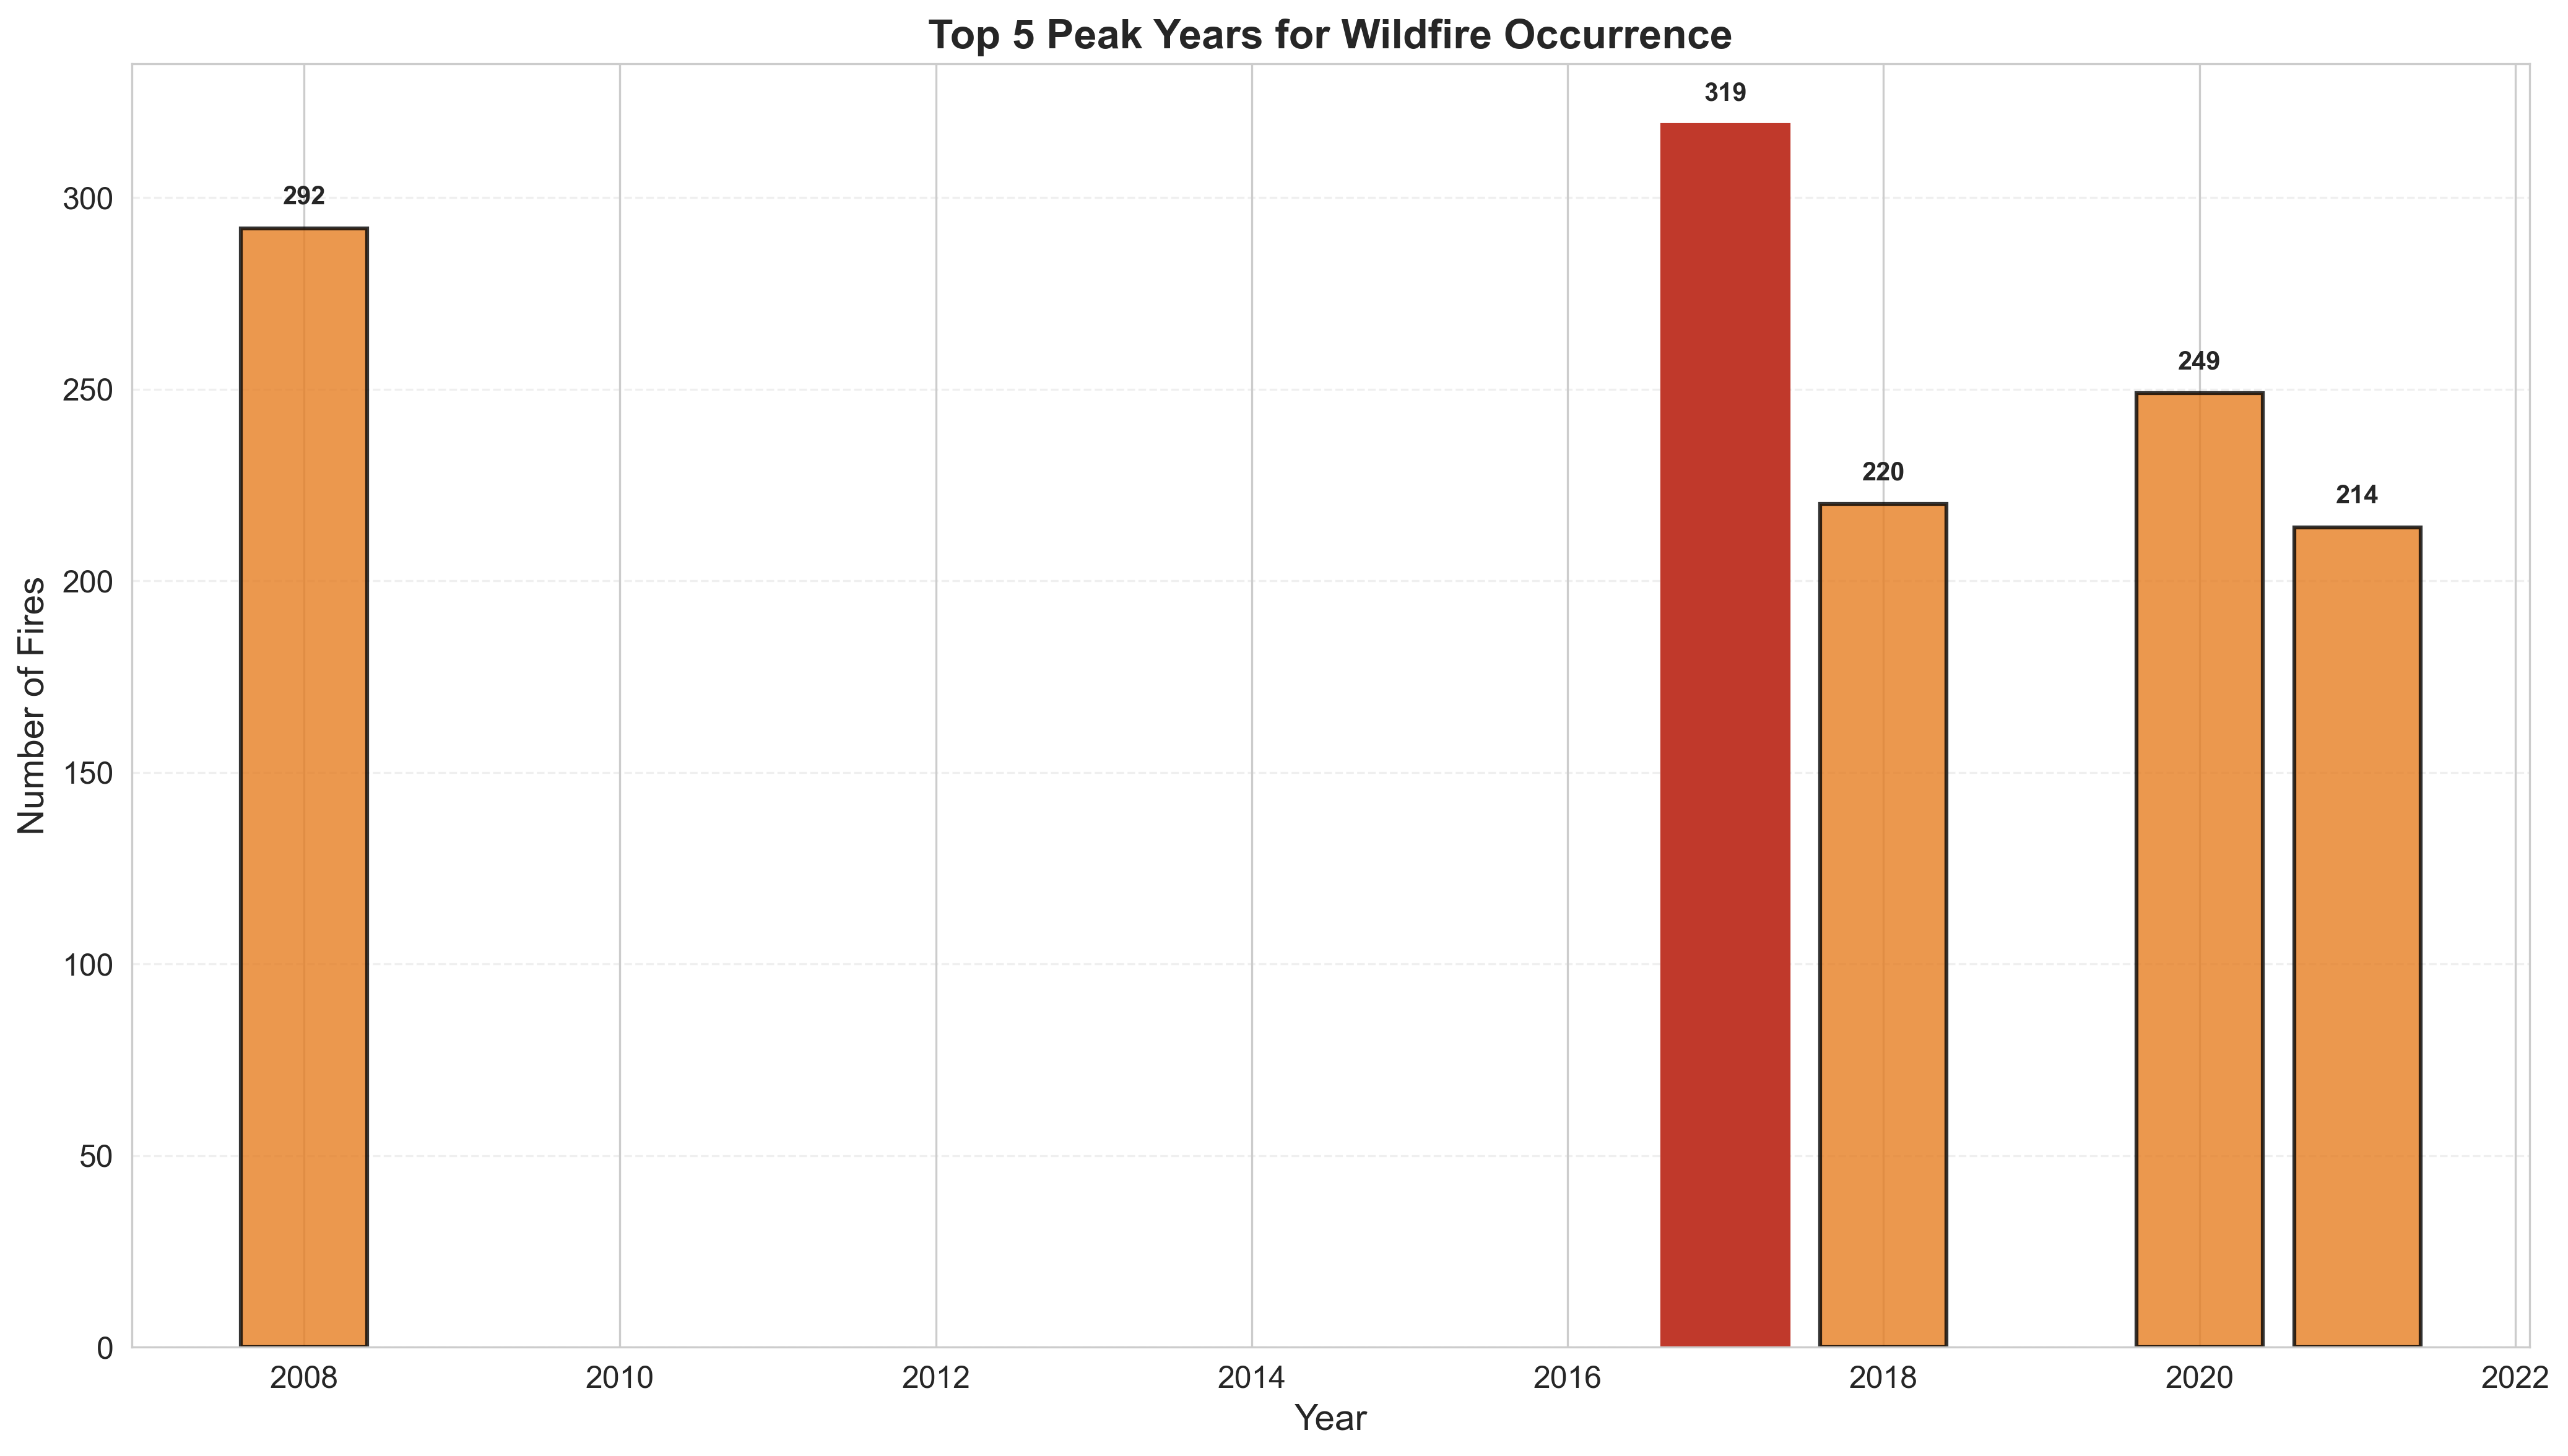
\includegraphics[width=0.85\textwidth]{peak_years_for_fires.png}
\caption{Top 10 peak years for wildfire occurrence. Note the dominance of recent years, with 2017 recording 319 fires---the highest in the 111-year dataset.}
\label{fig:peakyears}
\end{figure}

\begin{tcolorbox}[colback=warningcolor!10!white, colframe=warningcolor]
\textbf{Insight:} This isn't just climate change---it's also population growth in wildland-urban interface zones, forest management practices, and improved fire detection/reporting. The temporal trend is real, but the causal mechanisms are complex.
\end{tcolorbox}

\subsection{Seasonality: Summer and Early Fall Dominate}

Fire occurrence varies \textbf{significantly across months} (chi-square test: $\chi^2 = 1267$, $p < 0.001$).

\textbf{Peak fire season:} June, July, August (in that order)

This aligns with California's Mediterranean climate:
\begin{itemize}
    \item Hot, dry summers create ideal fire conditions
    \item Winter/spring rains reduce vegetation moisture
    \item Fall brings dry Santa Ana winds (Southern CA)
    \item Spring has increased activity (early-season fires)
\end{itemize}

\textbf{Policy implication:} Resource allocation should peak June--August, with sustained readiness through October.

\begin{figure}[h]
\centering
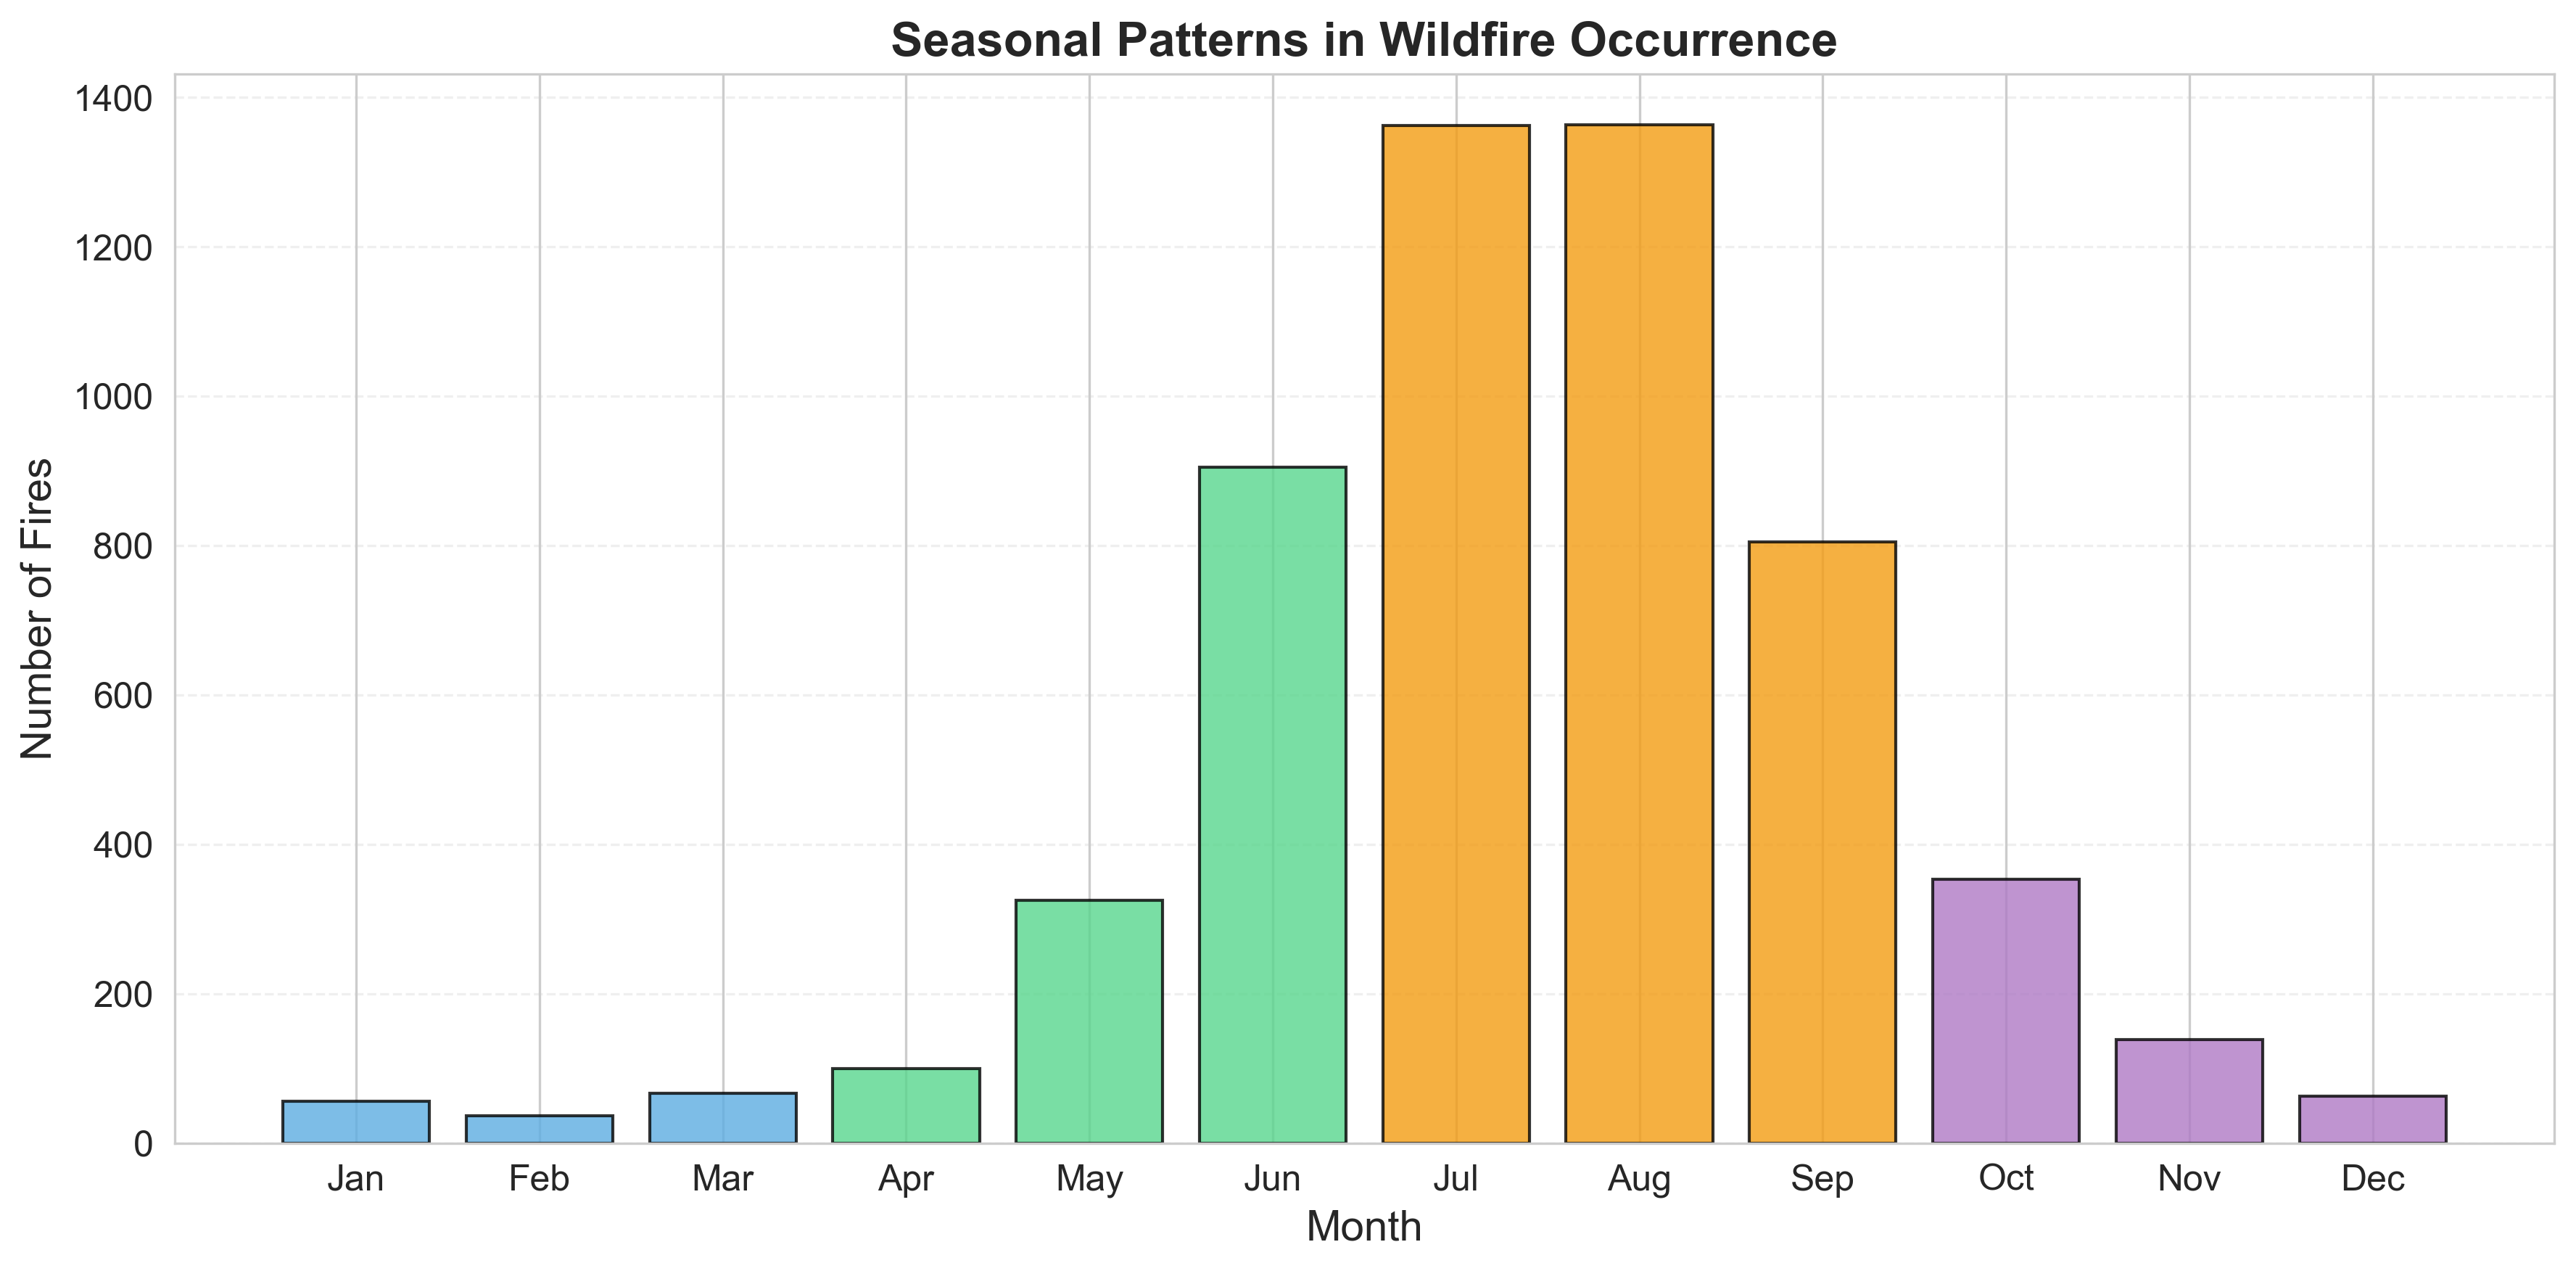
\includegraphics[width=0.85\textwidth]{seasonality.png}
\caption{Seasonal patterns in wildfire occurrence showing strong summer peak. Chi-square test confirms statistically significant variation across months ($p < 0.001$), with June, July, and August dominating.}
\label{fig:seasonality}
\end{figure}

\subsection{Fire Causes: Nature vs. Humans}

Analysis of ignition sources reveals a critical split:

\begin{center}
\begin{tabular}{lrr}
\toprule
\textbf{Cause} & \textbf{Count} & \textbf{\%} \\
\midrule
Lightning & 2,041 & 36.6\% \\
Unknown & 866 & 15.5\% \\
Miscellaneous & 714 & 12.8\% \\
Equipment Use & 432 & 7.8\% \\
Arson & 406 & 7.3\% \\
Debris Burning & 246 & 4.4\% \\
Campfire & 227 & 4.1\% \\
\textit{Other human causes} & \textit{643} & \textit{11.5\%} \\
\midrule
\textbf{Total} & \textbf{5,575} & \textbf{100\%} \\
\bottomrule
\end{tabular}
\end{center}

\textbf{Key finding:} While lightning is the single largest cause (36.6\%), \textbf{human-caused fires collectively account for $\sim$63\% of incidents} when excluding ``Unknown.''

\begin{tcolorbox}[colback=infocolor!10!white, colframe=infocolor]
\textbf{Insight:} This suggests prevention efforts targeting human behavior (equipment maintenance, campfire safety, debris burning regulations, arson prevention) could substantially reduce fire occurrence. Lightning is unavoidable; human error is preventable.
\end{tcolorbox}

\begin{figure}[h]
\centering
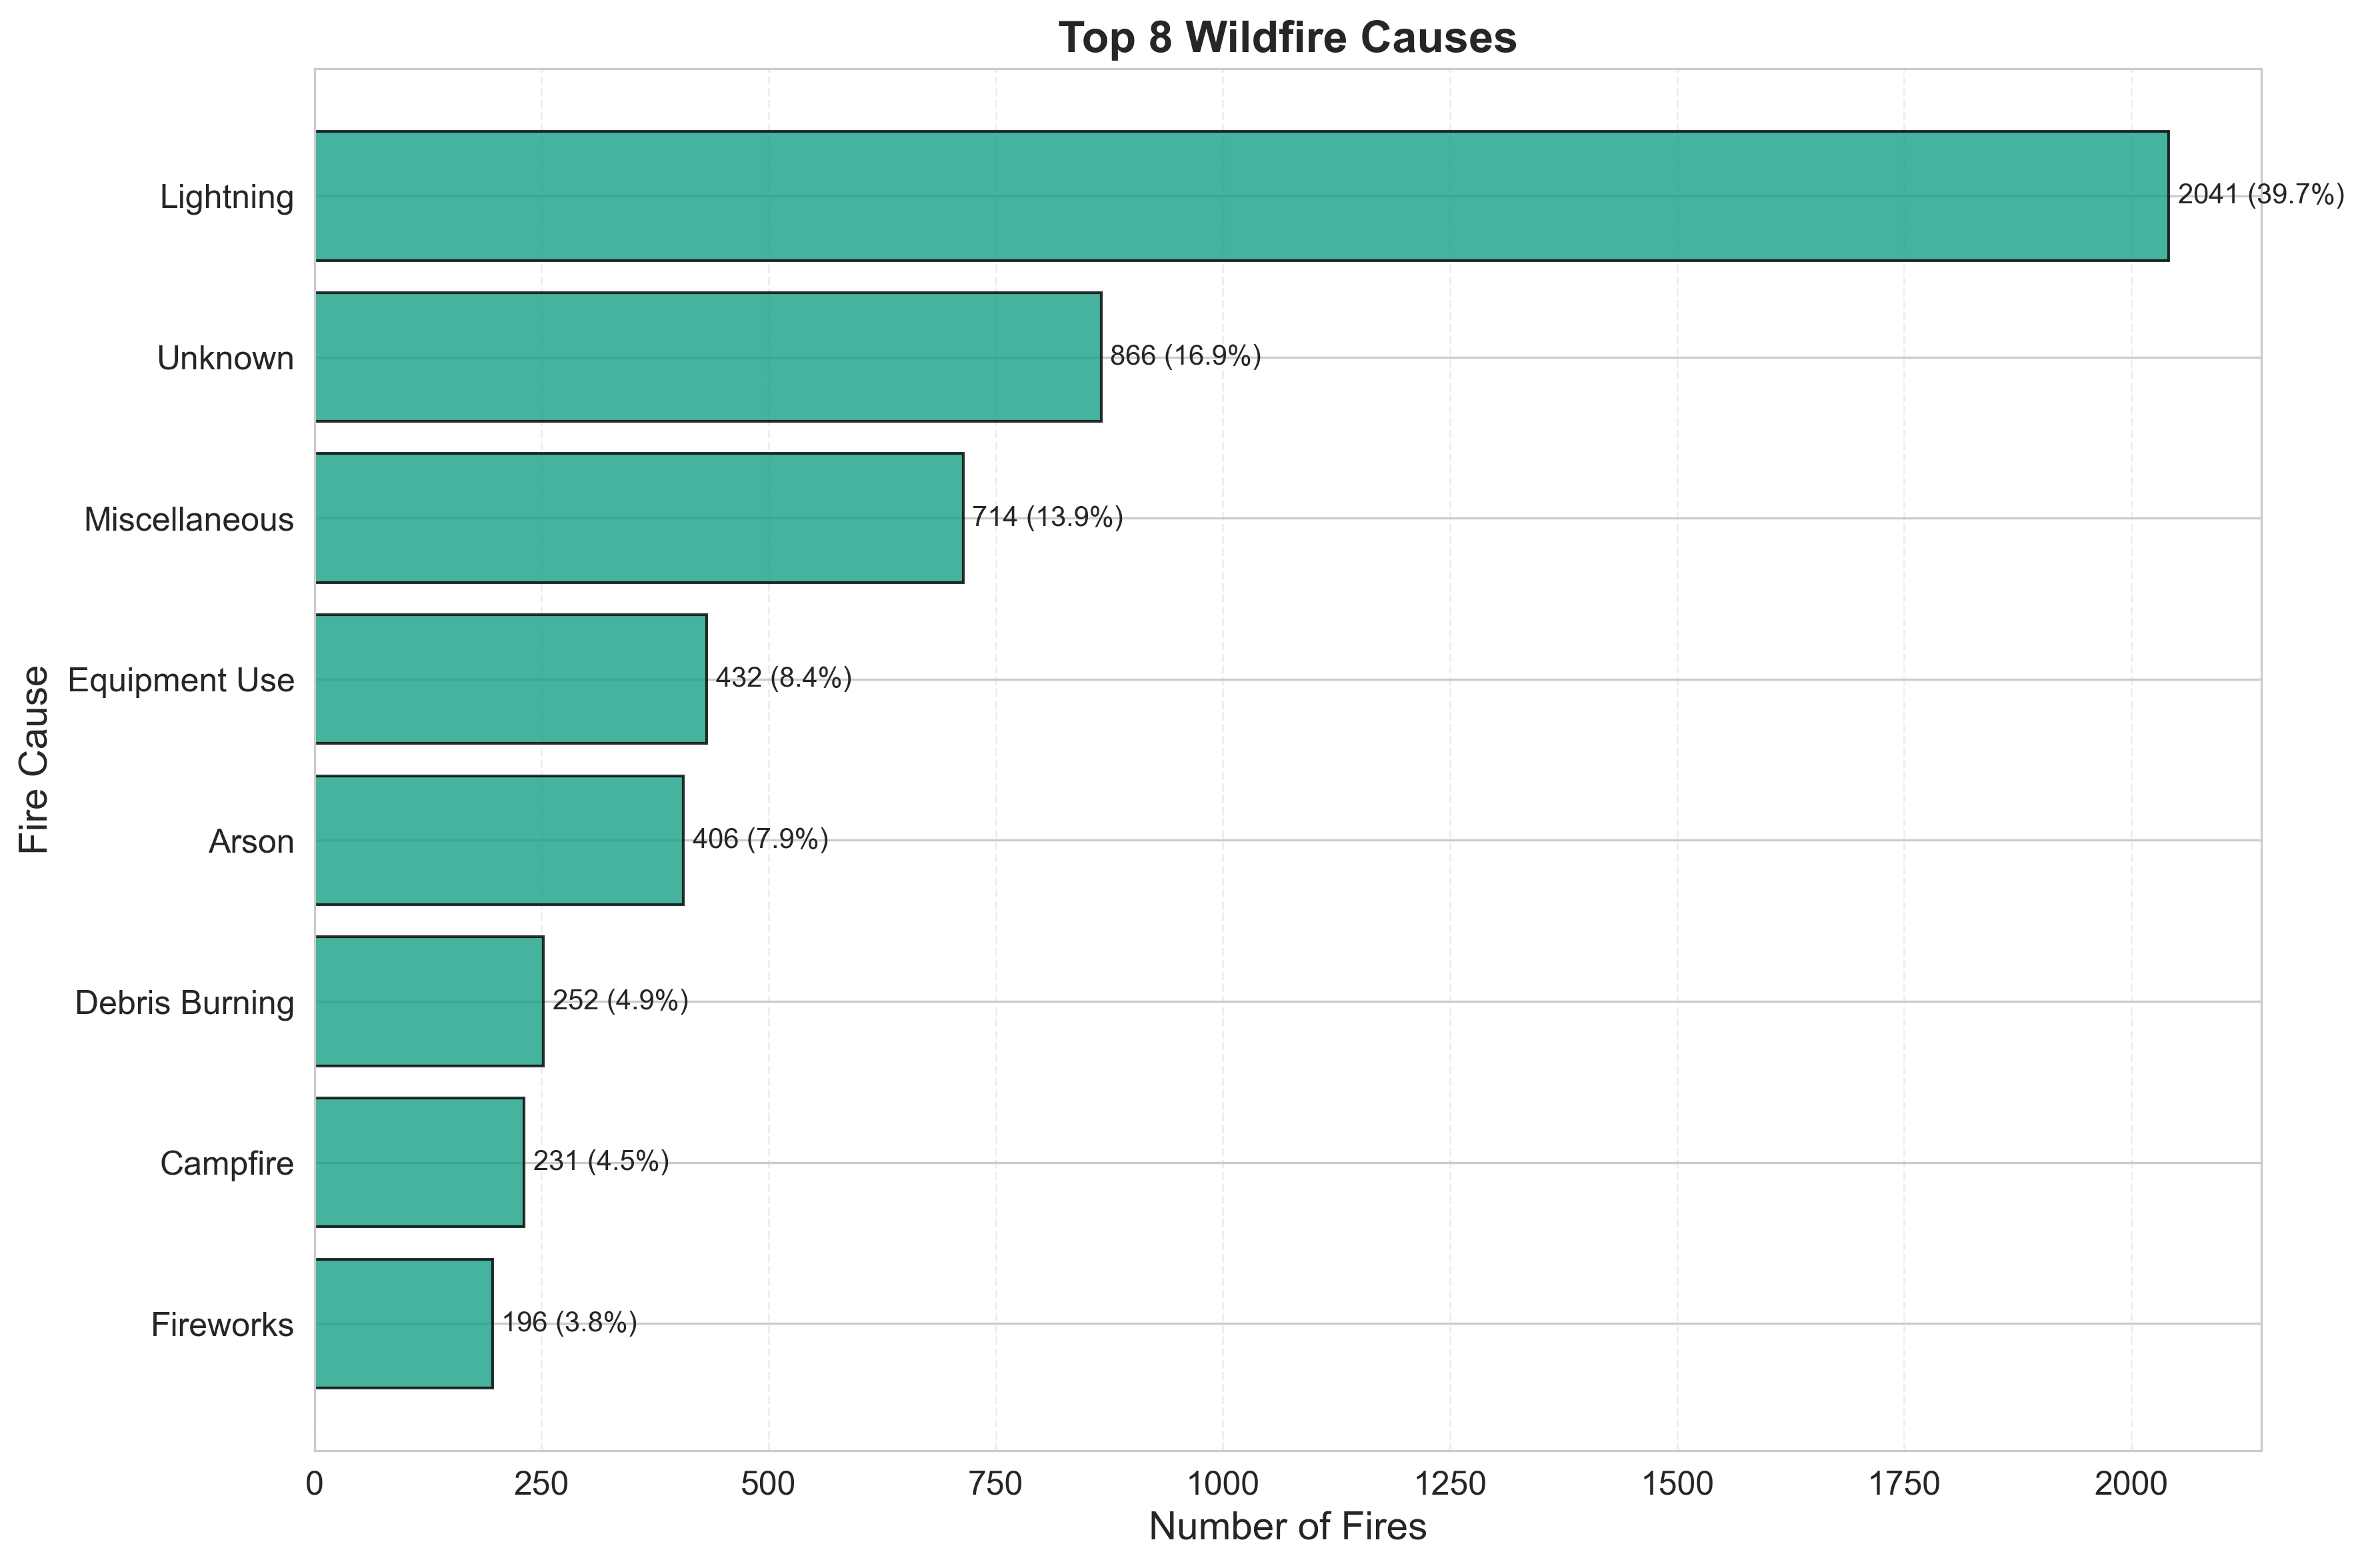
\includegraphics[width=0.85\textwidth]{cause_distribution.png}
\caption{Distribution of wildfire causes. Lightning dominates as a single source (36.6\%), but human-caused fires collectively represent the majority when excluding ``Unknown'' classification.}
\label{fig:causes}
\end{figure}

%=====================================
\section{The Containment Effectiveness Problem}
%=====================================

\subsection{What I Found Wrong}

Standard fire management analyses often use an ``effectiveness'' metric:

\begin{equation}
\text{Effectiveness} = \frac{\text{Fire Size (acres)}}{\text{Containment Duration (hours)}}
\end{equation}

This metric appears in reports, academic papers, and management assessments. \textbf{It is fundamentally flawed.}

\subsection{Why This Metric Fails}

The metric conflates \textbf{fire size} with \textbf{suppression quality}:

\begin{enumerate}
    \item \textbf{Larger fires naturally take longer to contain}, regardless of response quality
    \item The metric rewards methods used on large fires (high acres/hour)
    \item It penalizes methods used on small fires (low acres/hour)
    \item \textbf{No control for initial conditions}: weather, terrain, fuel load, resources available
\end{enumerate}

\textbf{Real-world analogy:} Imagine rating surgeons by ``patients treated per hour'' without distinguishing between removing a splinter and performing cardiac surgery. The metric would rank the splinter-removal doctor as ``more effective''---but that's absurd.

\subsection{What the Data Shows (With Caveats)}

Despite these limitations, ANOVA testing shows \textbf{statistically significant differences} between containment methods ($F = 14.54$, $p < 0.001$):

\begin{center}
\begin{tabular}{lrr}
\toprule
\textbf{Method} & \textbf{Effectiveness} & \textbf{Sample} \\
 & \textbf{(acres/hr)} & \textbf{Size} \\
\midrule
Aerial Suppression & 22.07 & $n=225$ \\
Mop-up Operations & 21.09 & $n=663$ \\
Indirect Attack & 20.53 & $n=454$ \\
Fire Shelter (Emergency) & 16.59 & $n=1,836$ \\
Fireline Construction & 14.56 & $n=49$ \\
\bottomrule
\end{tabular}
\end{center}

\begin{figure}[h]
\centering
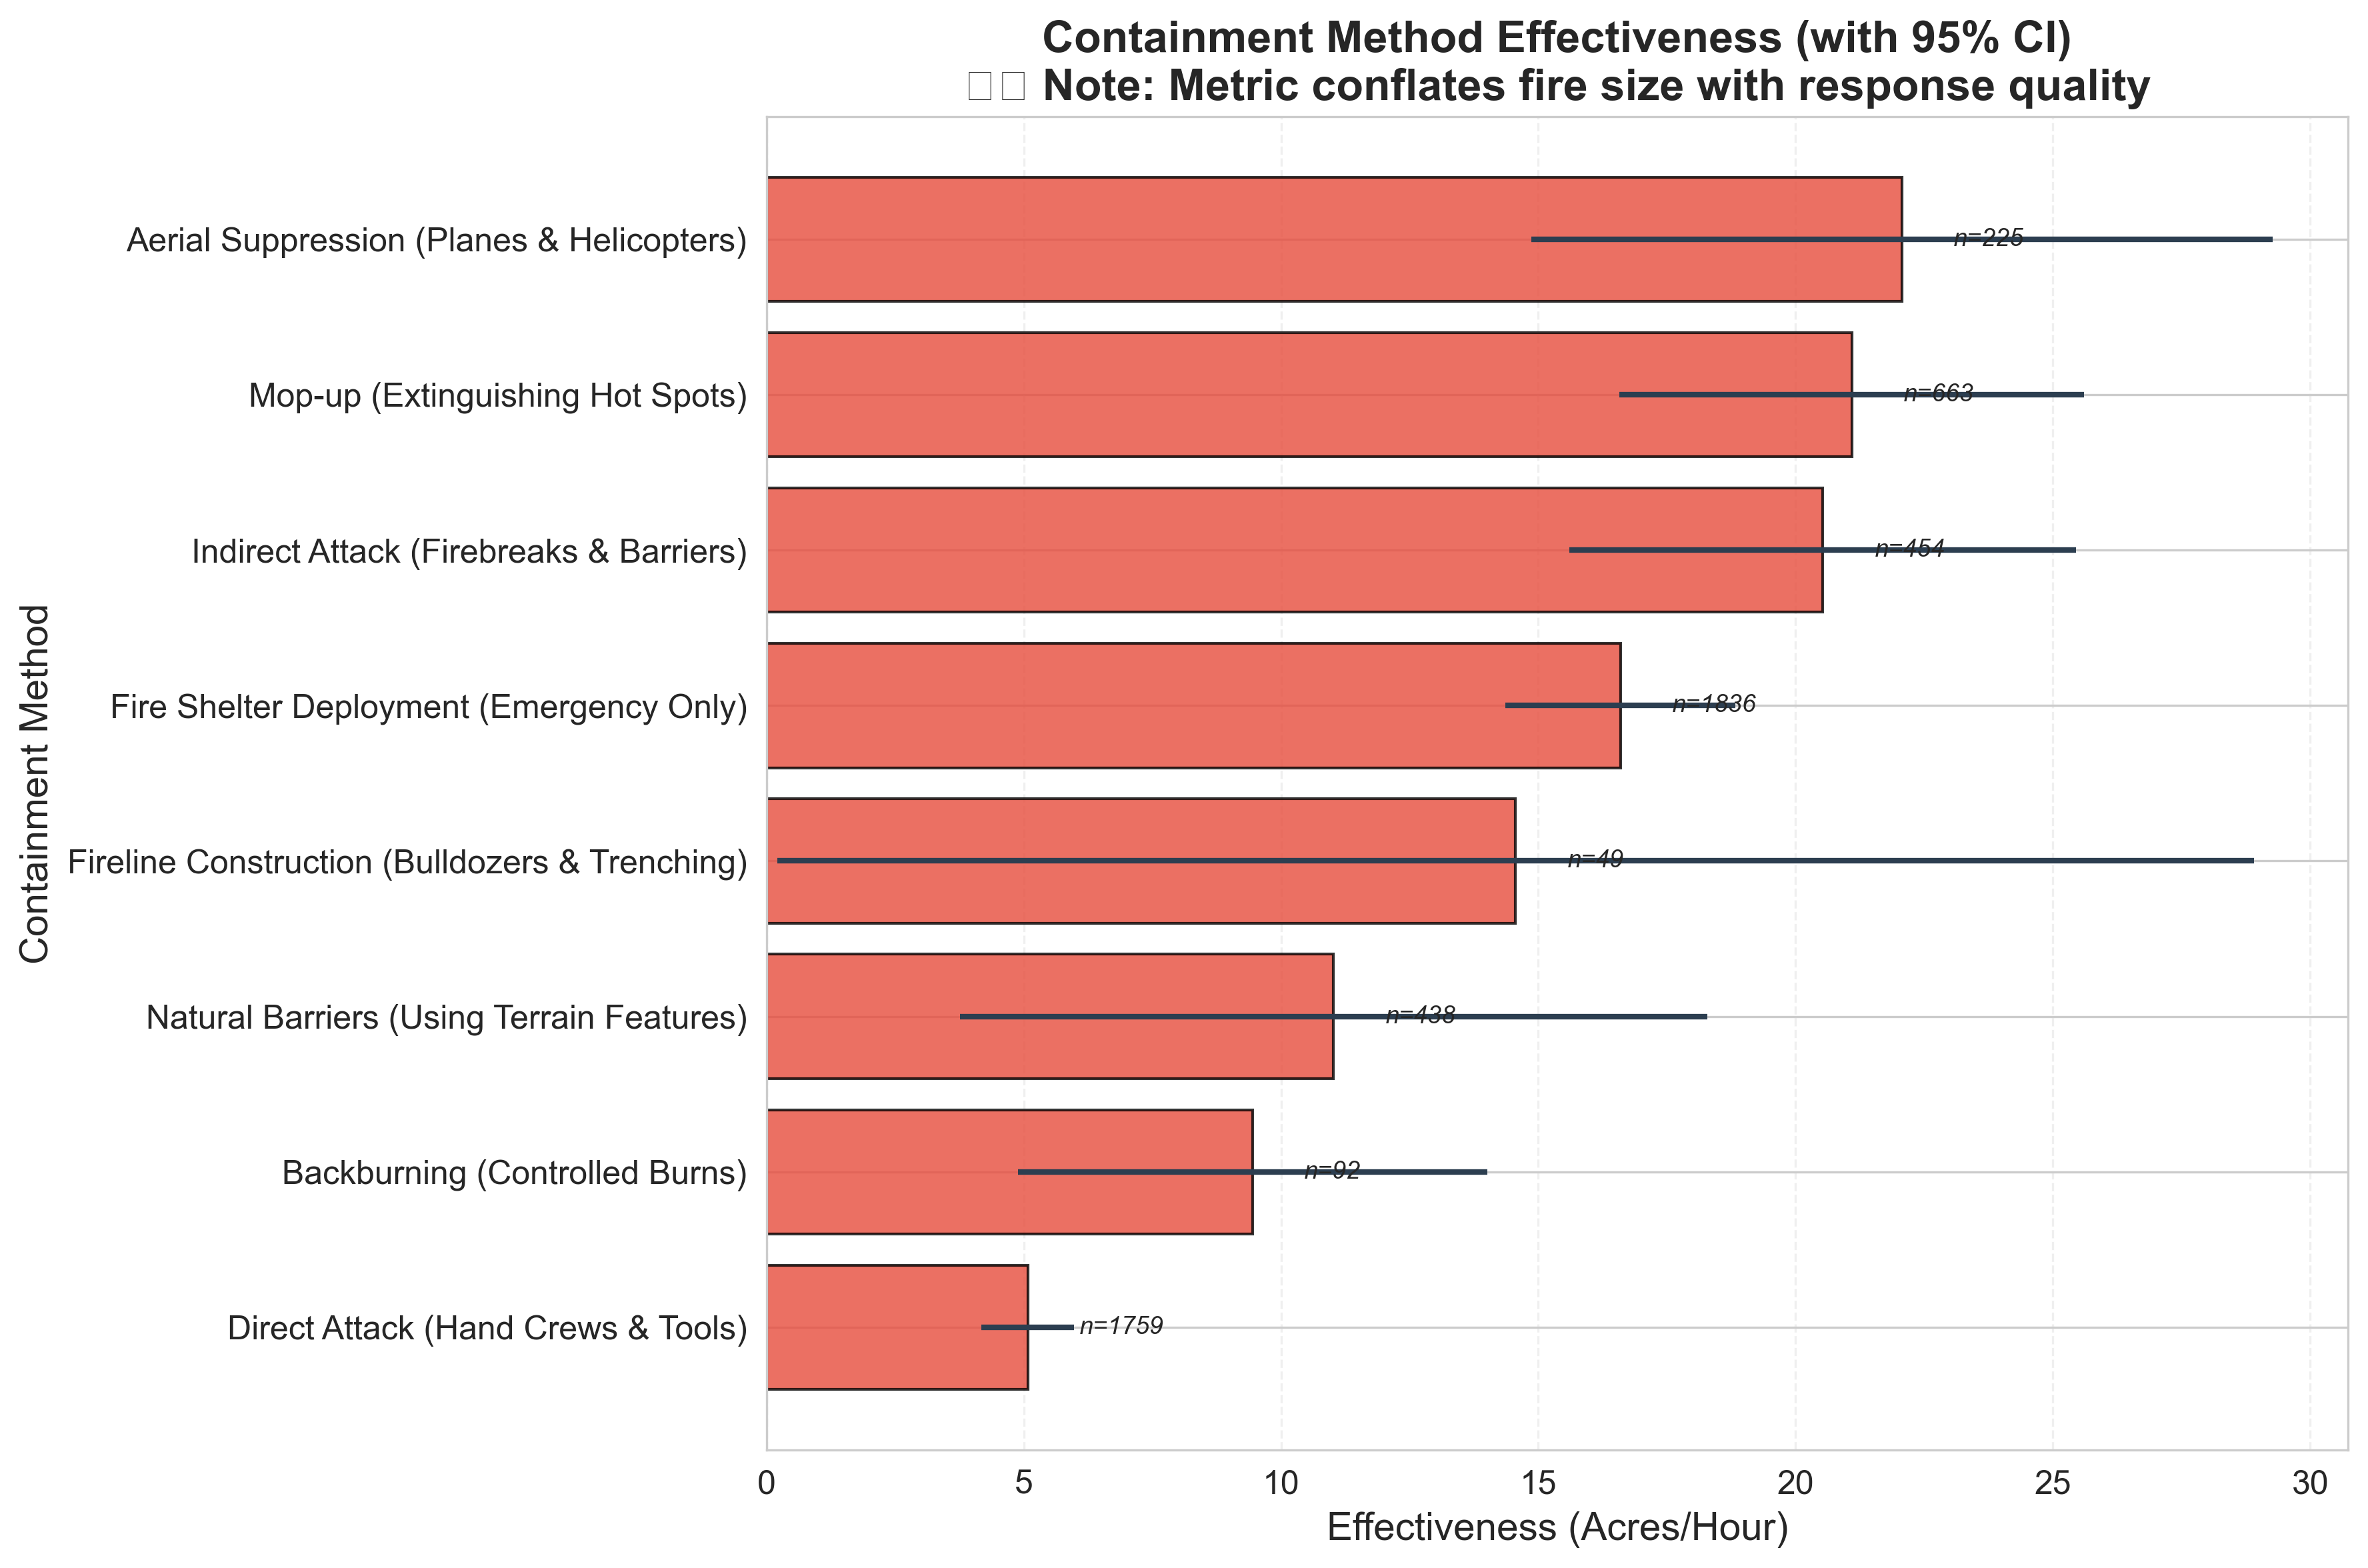
\includegraphics[width=0.9\textwidth]{containment_effectiveness.png}
\caption{Containment method ``effectiveness'' with 95\% confidence intervals. \textbf{Warning:} This metric conflates fire size with suppression quality and should not be interpreted as causal. Methods are not randomly assigned to fires---different methods are used in different contexts.}
\label{fig:effectiveness}
\end{figure}

\textbf{BUT}: These differences likely reflect \textbf{which methods are deployed on which types of fires}, not true effectiveness. Aerial suppression may rank high because it's reserved for large, accessible fires. Direct attack may rank low because it's used on small fires in rough terrain.

\begin{tcolorbox}[colback=warningcolor!10!white, colframe=warningcolor, title=\textbf{Critical Methodological Note}]
\textbf{I cannot make causal claims about method effectiveness from this data.} Containment methods are not randomly assigned to fires. Different methods are used in different contexts (fire size, terrain, weather, resources). Without controlling for these confounders, we're observing \textbf{correlations, not causation}.

\textbf{Honest limitation acknowledgment is essential for scientific integrity.}
\end{tcolorbox}

%=====================================
\section{How to Fix This}
%=====================================

To properly evaluate containment effectiveness, we need:

\subsection{1. Size-Controlled Metrics}

Normalize by initial fire size at detection:

\begin{equation}
\text{Growth Rate} = \frac{\text{Final Size} - \text{Initial Size}}{\text{Initial Size} \times \text{Duration}}
\end{equation}

This measures how much the fire grew relative to its starting point, controlling for the fact that large fires spread faster.

\subsection{2. Multiple Regression with Confounders}

Model containment duration while controlling for fire characteristics:

\begin{equation}
\text{Duration} = \beta_0 + \beta_1(\text{Size}) + \beta_2(\text{Weather}) + \beta_3(\text{Terrain}) + \beta_4(\text{Method}) + \epsilon
\end{equation}

This isolates the method's effect from other factors.

\subsection{3. Propensity Score Matching}

Match fires with similar initial characteristics but different methods, then compare outcomes. This mimics randomized controlled trials.

\subsection{4. Survival Analysis}

Use Cox proportional hazards models to analyze time-to-containment while accounting for censoring and time-varying covariates.

\subsection{5. Integrate Missing Variables}

Critical data needed:
\begin{itemize}
    \item \textbf{Weather:} Wind speed, humidity, temperature, precipitation
    \item \textbf{Terrain:} Slope, elevation, fuel type/load, accessibility
    \item \textbf{Resources:} Crew sizes, equipment deployed, budget allocated
    \item \textbf{Initial conditions:} Fire size at detection, rate of spread
\end{itemize}

These variables are available from NOAA, USGS, and fire management records---they just need to be integrated.

%=====================================
\section{What This Means for Policy}
%=====================================

\subsection{Actionable Insights}

\textbf{1. Prevention Focus on Human Causes}

With $\sim$63\% of fires human-caused, prevention programs targeting equipment maintenance, campfire safety, and arson reduction could substantially decrease fire occurrence.

\textbf{2. Resource Allocation by Season}

Peak staffing and equipment should align with June--August fire season, with sustained readiness through October.

\textbf{3. Prepare for Extremes, Not Averages}

The median fire is 127 acres; the 99th percentile is 83,193 acres. Planning for ``average'' fires is inadequate. Resource strategies must account for rare but catastrophic events.

\textbf{4. Improve Data Collection}

Current data lacks critical variables (weather, terrain, resources). Integrating these into fire incident reports would enable better causal inference and evidence-based policy.

\textbf{5. Method Evaluation Needs Better Metrics}

Current effectiveness measures are flawed. Fire agencies should adopt size-controlled metrics and rigorous statistical methods (propensity matching, survival analysis) before drawing conclusions about method superiority.

%=====================================
\section{The Path Forward}
%=====================================

This project establishes a foundation, but significant work remains:

\subsection{Immediate Next Steps}

\begin{enumerate}
    \item \textbf{Weather Data Integration:} Merge NOAA climate data with fire records
    \item \textbf{Spatial Analysis:} Examine geographic clustering and spread patterns using GIS
    \item \textbf{Predictive Modeling:} Build machine learning models for fire risk forecasting
    \item \textbf{Improved Metrics:} Implement size-controlled effectiveness measures
    \item \textbf{Sensitivity Analysis:} Test robustness of findings to analytical choices
\end{enumerate}

\subsection{Long-Term Research Agenda}

\begin{enumerate}
    \item \textbf{Causal Inference:} Use quasi-experimental designs (natural experiments, instrumental variables) to identify true causal effects of suppression methods
    \item \textbf{Real-time Risk Mapping:} Develop operational risk models integrating live weather, fuel moisture, and historical patterns
    \item \textbf{Cost-Benefit Analysis:} Evaluate suppression strategies by cost-effectiveness, not just containment speed
    \item \textbf{Climate Change Scenarios:} Model future fire patterns under different climate trajectories
\end{enumerate}

%=====================================
\section{Methodological Transparency}
%=====================================

\subsection{What Makes This Research Credible}

\textbf{1. Statistical Rigor}
\begin{itemize}
    \item Hypothesis testing with stated null hypotheses
    \item P-values and effect sizes reported
    \item 95\% confidence intervals on all estimates
    \item Appropriate tests selected (ANOVA, chi-square, linear regression, Kruskal-Wallis)
\end{itemize}

\textbf{2. Reproducibility}
\begin{itemize}
    \item All code open-source (\href{https://github.com/ngrief/FireAnalyst}{GitHub})
    \item Dependencies version-pinned (requirements.txt)
    \item Automated pipeline (one-command execution)
    \item Complete documentation (LaTeX methodology + code docstrings)
\end{itemize}

\textbf{3. Honest Limitations}
\begin{itemize}
    \item Effectiveness metric flaw prominently acknowledged
    \item Missing variables clearly stated
    \item Selection bias discussed
    \item Causal claims avoided where inappropriate
\end{itemize}

\textbf{4. Data Quality}
\begin{itemize}
    \item Six-stage validation framework
    \item 56.7\% data loss documented (not hidden)
    \item Outlier retention justified by domain knowledge
    \item Temporal reporting bias acknowledged
\end{itemize}

\subsection{Why Acknowledge Flaws?}

\textbf{Scientific integrity requires honesty about limitations.} Acknowledging the effectiveness metric flaw doesn't undermine this work---it strengthens it. It shows:

\begin{itemize}
    \item Critical thinking about causality vs. correlation
    \item Understanding of confounding variables and selection bias
    \item Commitment to truth over convenient narratives
    \item Professional research standards
\end{itemize}

The goal isn't to have perfect data or flawless methods. The goal is to \textbf{extract maximum insight from available data while being honest about constraints}.

%=====================================
\section{Conclusion}
%=====================================

This analysis of 111 years and 23 million acres of California wildfire data reveals:

\begin{enumerate}
    \item \textbf{Fire activity is significantly increasing}, particularly in the 21st century
    \item \textbf{Seasonality is pronounced}, with summer months dominating
    \item \textbf{Human causes are preventable}, representing $\sim$63\% of fires
    \item \textbf{Current effectiveness metrics are fundamentally flawed} and need replacement
    \item \textbf{Policy should focus on prevention, seasonal resource allocation, and preparing for extremes}
\end{enumerate}

More importantly, this project demonstrates how to conduct \textbf{rigorous, reproducible, and honest data analysis} on complex real-world problems. The identification and acknowledgment of methodological limitations---particularly the effectiveness metric flaw---exemplifies scientific integrity.

\subsection{The Bigger Picture}

California's wildfire challenge won't be solved by data analysis alone. It requires:
\begin{itemize}
    \item Climate change mitigation
    \item Forest management reform
    \item Building code enforcement
    \item Public education
    \item Sustained funding
\end{itemize}

But \textbf{evidence-based policy requires evidence}. This project provides a foundation for understanding patterns, evaluating methods, and guiding resource allocation---with intellectual honesty about what we know, what we don't know, and what we need to find out.

\vspace{0.5cm}

\begin{center}
\rule{0.8\textwidth}{0.4pt}

\textbf{Project Resources}

\vspace{0.2cm}

\href{https://github.com/ngrief/FireAnalyst}{\textbf{GitHub Repository:} github.com/ngrief/FireAnalyst}

Full source code, documentation, and LaTeX methodology

\vspace{0.2cm}

\textit{All analyses reproducible with a single command}
\end{center}

\end{document}